\documentclass[12pt,a4paper,twoside]{book}


\usepackage[utf8]{inputenc}
\usepackage[a4paper,inner=3.5cm,outer=2.5cm]{geometry}

\usepackage[titletoc,title,toc,page]{appendix}
\usepackage{verbatim}
\usepackage{placeins}
\usepackage{listings}
\usepackage{hyperref}
\usepackage[italian]{babel}
\usepackage{tikz}
\usepackage{parskip}
\usepackage{acronym}
\usepackage{notes}
\usepackage{graphicx}
\usepackage{blindtext}
\usepackage{chngcntr}
\counterwithin{table}{chapter}

\usepackage{newlfont}
\usepackage{fancyhdr}
\usepackage{indentfirst}
\usepackage[utf8]{inputenc}
\usepackage{float}
\usepackage{hyperref}
\usepackage[capitalize,noabbrev]{cleveref}
\usepackage{soul}
\usepackage[font=footnotesize,labelfont=bf]{caption}

\usepackage{multirow}
\usepackage{hyphenat}
\hyphenation{mate-mati-ca recu-perare}

\usepackage{lscape} 

\usepackage{natbib}
\bibliographystyle{alpha}
\setcitestyle{super, open={[}, close={]}}

\newcommand{\rom}[1]{\uppercase\expandafter{\romannumeral #1\relax}}

\usepackage{pdfpages}

\begin{document}
% Per spostare i vari elementi più su o più giù gioca con i valori di vspace che ci sono tra uno e l'altro
\pagestyle{empty}
\newgeometry{
    left=20mm,
    right=20mm,
    top=20mm,
    bottom=20mm
}

\begin{titlepage}

    \begin{center}

        % marchio di ateneo
        
\includegraphics[width=6.5cm,height=4.7cm]{img/marchio-di-ateneo.png}

        \vspace{10mm}

        % \large is 12pt
        {\large{\bf{Dipartimento d'Informatica - Scienza e Ingegneria}}}

        \vspace{5mm}

        % \Large is 14.4pt
        {\Large{\bf{Corso di Laurea in Ingegneria e Scienze Informatiche}}}

        \vspace{15mm}

        {\Huge{\bf Sviluppo e Ottimizzazione}}\\
        \vspace{3mm}
        {\Huge{\bf di un Sistema di Telemetria per Razzi}}\\
        % \vspace{3mm}
        % {\Huge{\bf  }}\\
        \vspace{3mm}
        {\Large{\bf Architettura e Trasmissione Dati con Tecnologia LoRa\textsuperscript{\copyright}}}
    \end{center}

    \vspace{50mm}

    \begin{minipage}[t]{0.40\textwidth}
        {\Large{\bf Relatore: \\ Chiar.mo Prof.\\ Andrea Piroddi}}

        \vspace{3mm}

        %{\Large{\bf Correlatore: \\ Chiar.mo Prof.\\ Nome Cognome}}
    \end{minipage}
    \hfill
    \begin{minipage}[t]{0.40\textwidth}\raggedleft
        {\Large{\bf Presentata da: \\ Alessandro Monticelli}}
    \end{minipage}

    \vspace{30mm}

    \rule[0.5cm]{15.8cm}{0.6mm}

    \begin{center}
        {\large{\bf Sessione luglio 2025 \\}}
        {\large{\bf Anno Accademico 2024/2025\\}}
    \end{center}

\end{titlepage}

\acrodef{IMU}{Inertial Measurement Unit}
\acrodef{IoT}{Internet of Things}
\acrodef{LoRa}[LoRa\textsuperscript{\textcopyright}]{Long Range}
\restoregeometry
\newpage
% \begin{center}
%     (DA FARE ALLA FINE)\\
%     5 parole chiave per caratterizzare il contenuto della dissertazione:\\ (se non ti piacciono così sparse puoi anche semplicamente scriverle su una riga sola)
% \end{center}

% % https://tex.stackexchange.com/questions/26538/words-scattered-randomly-in-on-coverpage
% \begin{tikzpicture}[overlay,remember picture,shift=(current page.center)]
% \pgfmathsetseed{3}


% \foreach [count=\count] \word in {Parola 1, parola 2, parola 3, parola 4, parola 5} {
% \node [
%     xshift={(mod(\count,3)-1)*(\paperwidth/4)},
%     yshift={(mod(\count,7)-3)*(\paperwidth/6)},
%     xshift=rand*4cm,
%     yshift=rand*2cm,
%     % rotate=rand*35,
%     % opacity=rnd*0.5+0.125,
%     font=\large] {\word};
% }
% \end{tikzpicture}
% \newpage

\topmargin=5.5cm
\begin{flushright}
    \emph{
        \LARGE{La dedica}\\\vspace{2mm}
        \LARGE{anche quella se vuoi}\\\vspace{3mm}
        \LARGE{su più righe}
    }
\end{flushright}
\newpage~\newpage
\pagenumbering{gobble}
\chapter*{Abstract}
Abstract qui (ti consiglio di farlo alla fine)

\topmargin=-1cm
\tableofcontents
\thispagestyle{empty}
\listoftables
\thispagestyle{empty}
\listoffigures
\thispagestyle{empty}
\newpage~\newpage


\pagenumbering{arabic}
\setcounter{chapter}{0}
\raggedbottom
\chapter{Introduzione} \label{chap:intro}
\pagestyle{plain}
\setcounter{page}{1}

\section{Presentazione del progetto Borealis di Aurora Rocketry.}
Aurora Rocketry è un'associazione studentesca dell'Università di Bologna nata 
nel 2024, che si occupa di progettare e costruire razzi sperimentali per 
partecipare a competizioni internazionali. \\
Borealis è il primo prototipo di razzo sperimentale sviluppato 
dall'associazione, progettato per raggiungere un'altitudine di 3Km.

Il razzo è formato da una sezione propulsiva (\emph{Motor bay}), una fusoliera 
in fibra di carbonio, divisa in \emph{Electronics bay}, \emph{Payload bay} e 
\emph{Parachute tube}, e un \emph{nose cone} per l'aerodinamica 
e l'espulsione del paracadute. \\
\begin{figure}[H]
    \centering
    % Se metti solo una delle due dimensioni, l'altra scala in automatico
    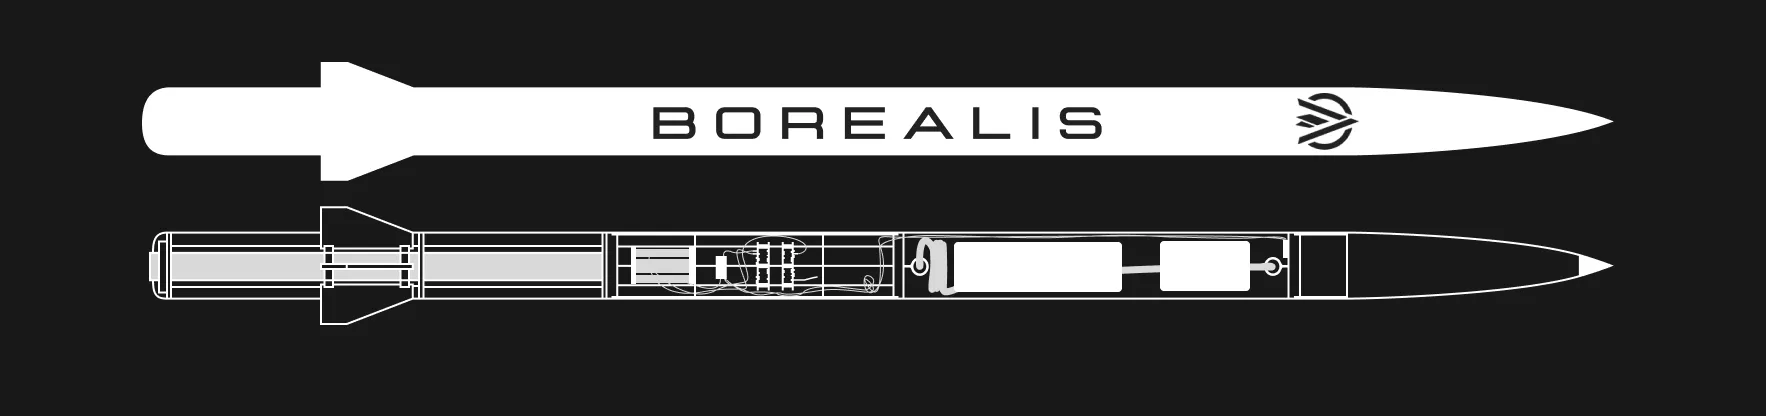
\includegraphics[width=10cm]{img/borealis-schema.png}
    \caption{Schema rappresentativo di \emph{Borealis}.}
    % La label ci vuole sempre e te la inventi tu: serve per riferirsi alle immagini successivamente
    \label{fig:borealis-schema}
\end{figure}

Nella \emph{Electronics bay} è presente il computer di volo, che si occupa di 
gestire il lancio e il recupero del razzo e di raccogliere dati durante il volo. \\
Il computer di volo è dotato di un sistema di telemetria che trasmette in tempo 
reale i dati raccolti a una \emph{ground station}, permettendo il monitoraggio 
del volo da terra.

\section{Contesto e importanza dei sistemi di telemetria nei razzi sperimentali.}
I razzi sperimentali occupano un ruolo fondamentale nella ricerca e nello 
sviluppo di tecnologie fin dalla fine del XIX secolo.

Originariamente usati per scopi militari fin dal XIII secolo, finch\'e tra il 
1926 e il 1929 il fisico americano Robert H. Goddard, grazie agli studi di 
Hermann Oberth e Konstantin Tsiolkovsky sulla velocità di fuga terrestre e la 
propulsione a razzo, realizz\`o il primo razzo a propellente liquido per scopi 
scientifici\cite{seibert2006history}.

Da allora, i razzi sperimentali sono stati utilizzati per una vasta gamma di 
applicazioni, tra cui:
\begin{itemize}
    \item La ricerca spaziale e l’esplorazione planetaria, con missioni come 
    i razzi-sonda impiegati per esperimenti scientifici in microgravità.
    \item Lo studio dell’atmosfera e dei fenomeni meteorologici, come i razzi 
    impiegati per analizzare la composizione degli strati superiori 
    dell’atmosfera terrestre.
    \item Il test di nuove tecnologie aerospaziali, inclusi materiali innovativi
     e sistemi di propulsione sperimentali.
    \item Applicazioni educative e accademiche, che permettono a università e 
    centri di ricerca di sviluppare esperimenti e formare studenti nel campo 
    dell’ingegneria aerospaziale.
\end{itemize}

Le motivazioni per cui \`e importante sviluppare un sistema di telemetria per un 
razzo sperimentale sono molteplici.

In primo luogo, il monitoraggio del volo in tempo reale permette di avere un 
\emph{feedback} immediato sulle prestazioni del razzo, sulle condizioni 
ambientali e sulle eventuali anomalie che possono verificarsi durante il volo.
Inoltre, la raccolta di dati durante il volo \`e fondamentale per l’analisi 
post missione e per l’ottimizzazione del design del razzo.
Infine, la telemetria \`e essenziale per poter analizzare il volo in caso di 
problemi o incidenti, al fine d'identificare le cause se il sistema di 
\emph{logging} a bordo dovesse andare perso.

Ciò pone delle sfide tecniche significative tra cui:
\begin{itemize}
    \item L'affidabilità della trasmissione dati, che deve essere mantenuta 
    nonostante le condizioni critiche a cui il sistema è soggetto, tra cui 
    accelerazioni estreme, eventi atmosferici e interferenze elettromagnetiche.
    \item L'ottimizzazione della raccolta dati, che deve avvenire in tempo reale
     e con una frequenza sufficiente per garantire la precisione delle misurazioni.
    \item La gestione del consumo energetico, che deve essere minimizzato per 
    garantire l'autonomia del sistema durante il volo.
\end{itemize}

\section{Obiettivi della tesi e contributo personale.}
L'obiettivo di questa tesi è la descrizione delle fasi di progettazione, 
sviluppo e ottimizzazione del sistema di telemetria per il razzo Borealis di 
Aurora Rocketry, offrendo una panoramica dettagliata delle tecnologie utilizzate 
e delle scelte progettuali effettuate, valutando le prestazioni del sistema e 
identificando possibili miglioramenti futuri.
Si vuole inoltre fornire un confronto tra le soluzioni adottate da Aurora 
Rocketry e quelle utilizzate in progetti simili, al fine di valutare l'impatto 
del sistema sviluppato nell'ambito della ricerca e dello sviluppo di razzi 
sperimentali.

Il mio contributo personale al progetto ha riguardato tutte le fasi di sviluppo 
del computer di volo, dal design iniziale alla realizzazione del prototipo, fino 
alla fase di test e ottimizzazione.
Ho contribuito alla scelta delle tecnologie utilizzate, alla progettazione 
dell'architettura del computer di volo e del sistema di telemetria e alla 
scrittura del software per la raccolta, la strutturazione e la trasmissione dati.
Inoltre, ho partecipato attivamente alle prove sperimentali e all'analisi dei 
dati raccolti, apportando modifiche e ottimizzazioni al sistema in base ai 
risultati ottenuti.

\chapter{Descrizione del Computer di Volo} \label{chap:flight-computer}

\section{Architettura del computer di volo Borealis.}
Il computer di volo di Borealis è basato su un microcontrollore ESP32-S3, montato
su una scheda di sviluppo Arduino Nano ESP32, un modulo di raccolta dati contenente
i sensori e un modulo per la telemetria contenente la ricetrasmittente \ac{LoRa}
e un modulo di attuatori per l'apertura del \emph{nose cone} tramite cariche
pirotecniche e la conseguente apertura dei paracadute per il recupero del razzo.

\subsection{Raccolta dati}
I sensori utilizzati sono:
\begin{itemize}
    \item Una \ac{IMU} \emph{Bosch BNO055} (Giroscopio, Accelerometro e Magnetometro).
    \item Due barometri \emph{Adafruit MPRLS} con presa statica.
\end{itemize}

\subsection{Telemetria}
Per la telemetria è stato impiegato un modulo \ac{LoRa} \emph{EByte E220 LLCC68}
a 868MHz, con un'antenna a dipolo e un amplificatore di potenza integrato ad
alta efficienza. \\

\section{Funzioni principali e componenti chiave.}
Il computer di volo si occupa del monitoraggio del volo. Tramite algoritmi
di \emph{sensor fusion} e \emph{data fusion} elabora i dati raccolti dai sensori
per ottenere informazioni sulla posizione, l'orientamento e la velocità del razzo.
In particolare fa uso di un Extended Kalman Filter per filtrare i dati rumorosi
dell'\ac{IMU} e dei due barometri, ottenendo una stima dell'orientamento, velocità
e altitudine del razzo.

Un algoritmo di rilevamento dell'apogeo permette di identificare il punto di massima
altezza raggiunto dal razzo, tenendo conto della variazione di altitudine, velocità
e direzione dell'accelerazione, attivando la sequenza di recupero.

\section{Integrazione e ruolo del sistema di telemetria.}

\chapter{Tecnologia \texorpdfstring{LoRa\textsuperscript{\textcopyright}} e la sua Applicazione} \label{chap:lora}

\section{Panoramica della tecnologia \texorpdfstring{LoRa\textsuperscript{\textcopyright}}.}
\cite{Andrade2022}
\section{Specifiche tecniche dei moduli utilizzati.}
\section{Motivazioni della scelta di \texorpdfstring{LoRa\textsuperscript{\textcopyright}} per il progetto.}

\chapter{Implementazione del Sistema di Telemetria} \label{chap:telemetry}

\section{Architettura del sistema di trasmissione dati.}
\section{Protocollo di comunicazione e gestione dati.}
\section{Implementazione software e algoritmi di gestione della trasmissione.}

\chapter{Valutazione delle Prestazioni} \label{chap:performance}

\section{Metodologia di test e criteri di valutazione.}
\section{Confronto tra simulazioni e risultati sul campo.}
\section{Ottimizzazioni apportate durante lo sviluppo.}

\chapter{Risultati e Analisi} \label{chap:results}

\section{Analisi dei dati raccolti durante le prove sperimentali.}
\section{Limiti e possibili miglioramenti futuri.}
\section{Implicazioni del sistema sviluppato per progetti simili.}

\chapter{Conclusioni} \label{chap:conclusion}

\section{Riepilogo dei risultati ottenuti.}
\section{Riflessioni sull'impatto del progetto nell'ambito della ricerca e dello sviluppo di razzi sperimentali.}
\section{Prospettive di sviluppo futuro.}

\renewcommand{\appendixtocname}{Appendici}
\renewcommand{\appendixpagename}{Appendici}
% \csname @openrightfalse\endcsname
\pagenumbering{gobble}
\begin{appendices}
    \chapter{Appendice A}
    \label{Appendice:A}
    Probabilmente ci sono un sacco di package non utilizzati ma così funziona tutto quindi non ho indagato oltre.

    Inoltre su internet c'è un sacco di documentazione se ti servisse.
    \chapter{Appendice B}
    \label{Appendice:B}
    Appendice B se serve

    \chapter{Embed di interi PDF}
    \label{Appendice:C}
    Se ti serve puoi fare embed di PDF interi con pdfpage, scegliendo anche le pagine (o mettendo - se le vuoi tutte):

    % 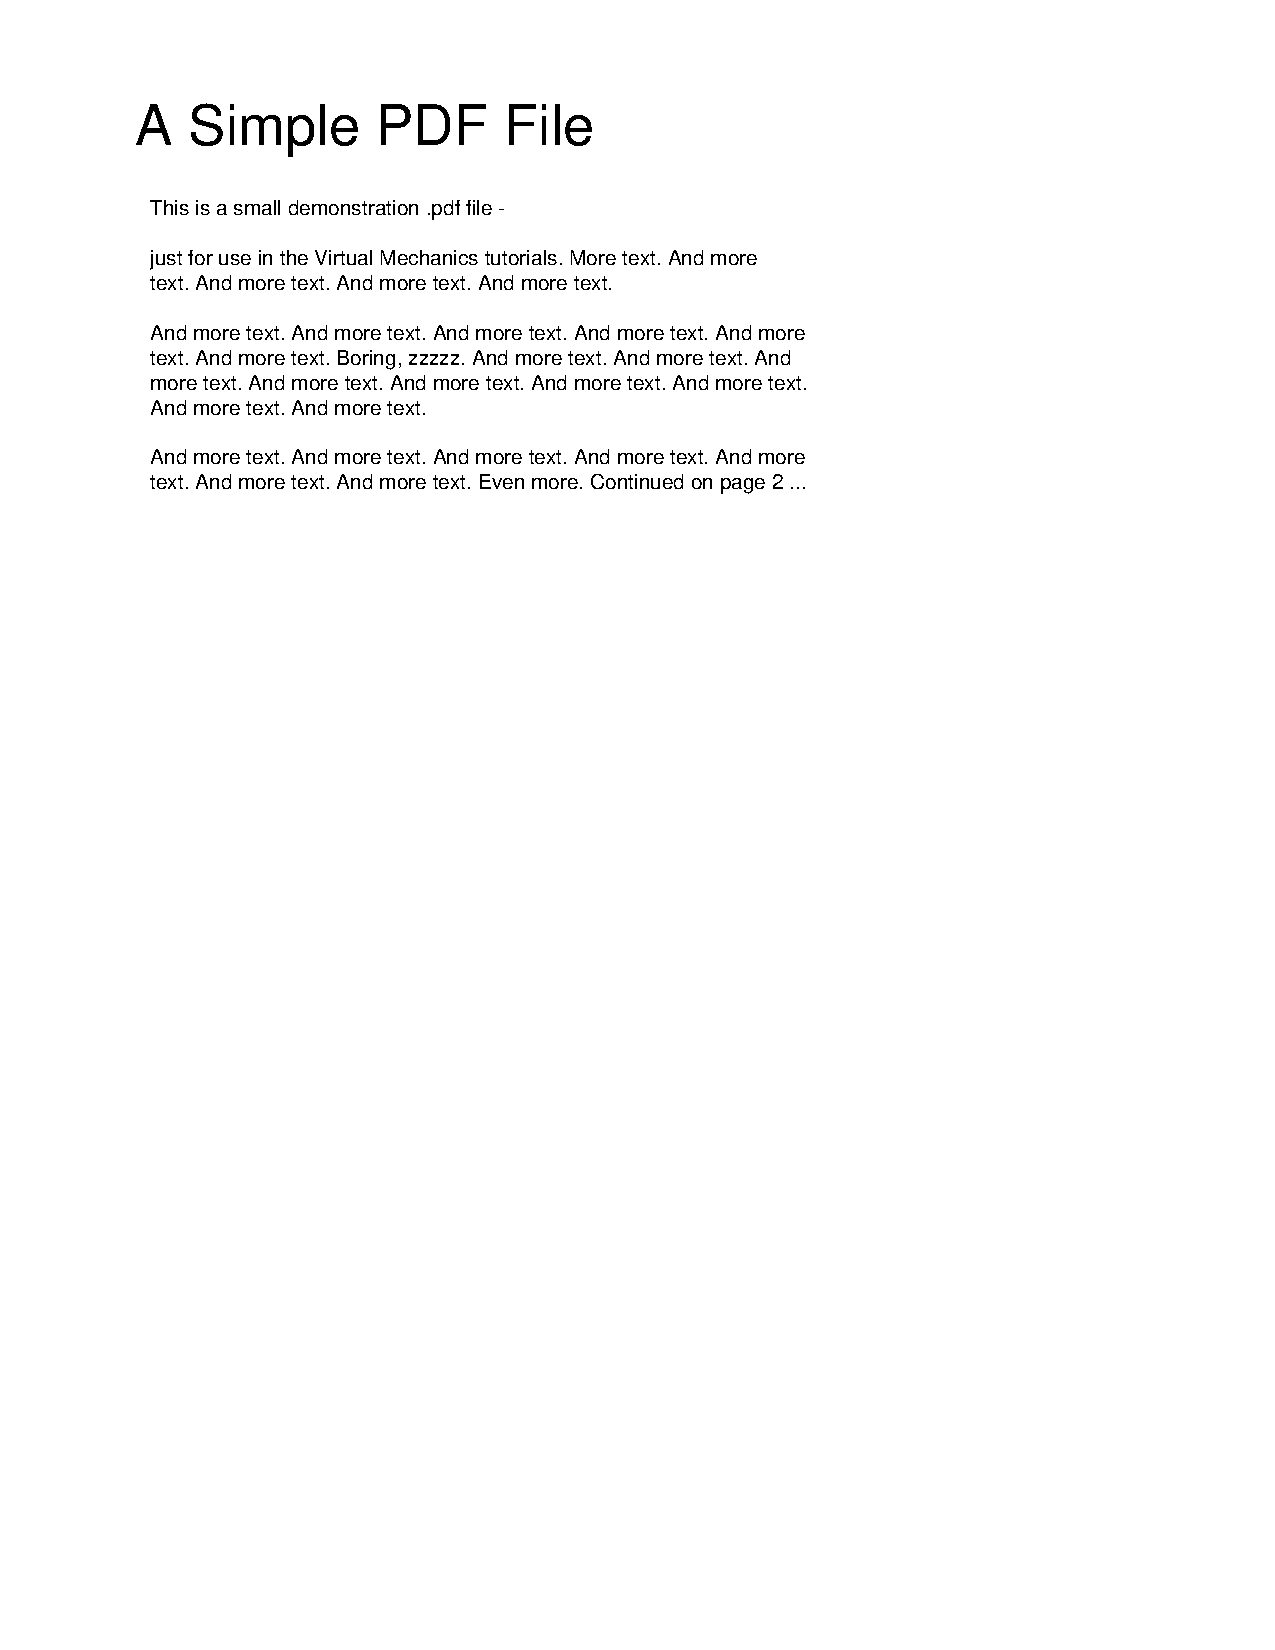
\includepdf[pages=1]{pdf/sample.pdf}
\end{appendices}
% \section{elenchi}
% \subsection{Elenchi puntati}
% \begin{itemize}
%     \item bla
%     \begin{itemize}
%         \item sub-bla
%     \end{itemize}
%     \item bla
% \end{itemize}

% \subsection{Elenchi numerati}
% \begin{enumerate}
%     \item bla1
%     \begin{enumerate}
%         \item sub bla 1
%         \item sub bla 2
%     \end{enumerate}
%     \item bla 2
% \end{enumerate}

% \subsection{Mix}
% \begin{itemize}
%     \item bla
%     \begin{enumerate}
%         \item sub bla 1
%     \end{enumerate}
%     \item bla
% \end{itemize}

% \begin{enumerate}
%     \item bla 1
%     \begin{itemize}
%         \item sub bla
%     \end{itemize}
%     \item bla 2
% \end{enumerate}

% \section{Font}
% \textbf{bla bla bla}\\
% \textit{Ancora bla bla bla}\\
% \texttt{bla bla ma in un'altra riga}

% \subsection{Sottosezione 1 - parskip}
% Grazie al package parskip se vai a capo nel .tex lasciando una riga

% ti mette un po' di spazio anche nel pdf.\\
% Attenzione però che ogni tanto questa feature fa lasciare troppo spazio tra testo e immagini / tabelle, se capita prova a togliere un po' di righe vuote. \\
% Senza questo pacchetto, una doppia new line (\texttt{$\backslash n\backslash n$}) crea un nuovo paragrafo, la cui prima riga viene leggermente indentata (un comportamento indesiderato se vieni da altri strumenti di stesura). Eventualmente, si può usare per allungare di qualche pagina alla tesi, evitando di abusarne.
% \subsection{Sottosezione 2 - capitoli}
% I capitoli iniziano sempre in una pagina dispari, quindi a volte vedrai delle pagine bianche tra uno e l'altro
% \subsubsection{Sottosottosezione 1} \label{subsub:bla}
% bla bla bla

% \chapter{Dopo l'introduzione}
% qua scrivi qualcosa
% \section{Immagini}
% Quando fai begin figure, ricordati di mettere tra quadre un modificatore di posizione: H significa esattamente nel punto dove si trova l'immagine nel file .tex e ti consiglio di usare quello, se no ci sono ad esempio t (top) e b (bottom).

% \begin{figure}[H]
%     \centering
%     % Se metti solo una delle due dimensioni, l'altra scala in automatico
%     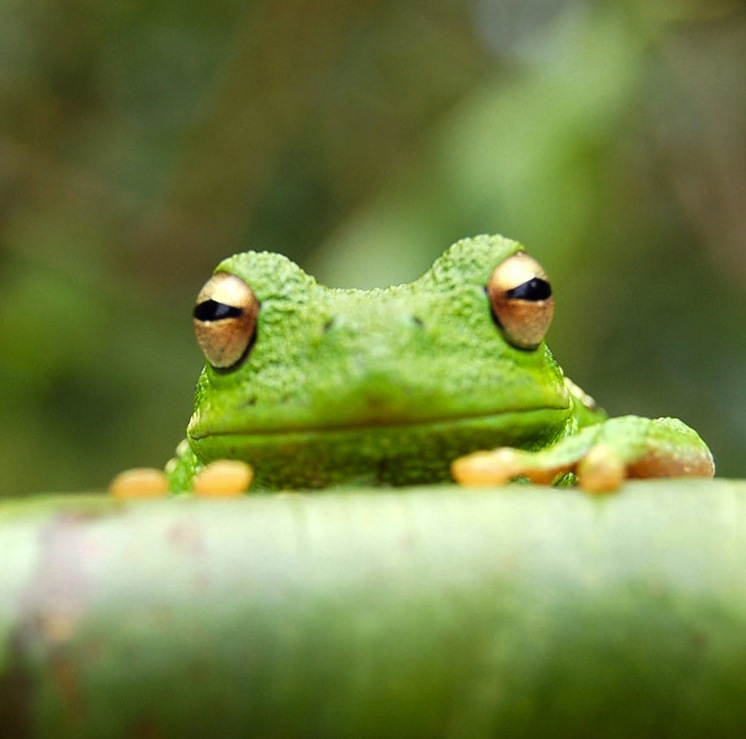
\includegraphics[height = 6cm, width=8cm]{img/frog.jpg}
%     \caption{Caption (questo viene scritto nell'indice delle figure)}
%     % La label ci vuole sempre e te la inventi tu: serve per riferirsi alle immagini successivamente
%     \label{fig:frog}
% \end{figure}

% \section{tabelle}
% \subsection{Tabella semplice}
% Anche qui nota H tra quadre, la caption e la label

% \begin{table}[H]
%     \centering
%     \begin{tabular}{|c|c|}
%     \hline
%         \textbf{Pratiche agili} & \textbf{Studenti}  \\ \hline
%         Sprint planning & 73  \\ \hline
%         Pair programming & 73  \\ \hline
%         Retrospettiva & 48  \\ \hline
%     \end{tabular}
%     \caption{Tabella semplice (anche questo scritto nell'indice delle tabelle)}
%     \label{tab:simple}
% \end{table}

% \subsection{tabelle avanzate}
% Con multirow (e multicolumn che però serve meno) puoi fare righe (colonne) più grandi del normale.\\
% \begin{table}[H]
%     \centering
%     \begin{tabular}{|c|c|c|c|c|}
%     \hline
%         \textbf{Team} & \textbf{LoC verificate} & \textbf{LoC sviluppatori} & \textbf{Ore sviluppatori} & \textbf{LoC/h}  \\ \hline
%         \multirow{2}*{1} & 1148& m: 888& m: 40& 22\cr & Diff: -1852& $\sigma$: 371& $\sigma$: 27& \\ \hline
%         \multirow{2}*{2}&1858& m: 1404& m: 65& 22\cr &  Diff: -448& $\sigma$: 1222& $\sigma$: 78& \\ \hline
%         \multirow{2}*{3}&1640& m: 1400& m: 96& 15\cr &  Diff: -2810& $\sigma$: 1417& $\sigma$: 41& \\ \hline
%     \end{tabular}
%     \caption{CAPTION}
%     \label{tab:avanz}
% \end{table}

% \subsubsection{Tabelle girate}
% Se usi landscape la tabella viene girata (nel caso dovessi inserirne una molto grande)
% \begin{landscape}
% \begin{table}[H]
%     \centering
%     \begin{tabular}{|c|c|}
%     \hline
%         \textbf{Numero} & \textbf{\#}  \\ \hline
%         UNO & 1  \\ \hline
%         DUE & 2  \\ \hline
%         TRE & 3  \\ \hline
%     \end{tabular}
%     \caption{Tabella girata}
%     \label{tab:girata}
% \end{table}

% \end{landscape}

% \section{Grafici}
% Puoi creare grafici con tikzpicture.
% Qui c'e' un grafico con asse x e y customizzabili per ogni tipo d'utilizzo.
% Tutti i tool e tutorial necessari per creare ogni tipo di grafico puo' essere trovato qui: https://tikz.dev/

% \begin{tikzpicture}
%   % Draw x-axis
%   \draw[->] (-1,0) -- (15,0) node[right] {$x$};
%   % Draw y-axis
%   \draw[->] (0,-1) -- (0,5) node[above] {$y$};

%   % Draw grid lines (optional)
%   \foreach \x in {1,2,3,4,5,6,7,8,9,10,11,12,13,14}
%     \draw (\x,-0.1) -- (\x,0.1);
%   \foreach \y in {1,2,3,4}
%     \draw (-0.1,\y) -- (0.1,\y);

%   % Draw origin
%   \fill (0,0) circle[radius=2pt];
% \end{tikzpicture}

% \section{Import di file TeX}
% Puoi importare altri file tex per intero includendoli cosi'.
% Questo e' molto utile per mettere insieme diversi capitoli di una tesi o di un grande documento in generale.

% Questo e' il contenuto del documento imported\textunderscore document.tex


% \chapter{Altri comandi}
% bla bla
% \section{Math mode}
% Per inserire simboli matematici (e lettere greche) serve la math mode:

% Usando il simbolo del dollaro hai la math mode inline: $5 \times \alpha = 3\lambda$

% Altrimenti hai quella con le barre e le quadre \[ \frac{\sum_6^i 3i\theta}{12k^2\times 7}\]

% Infine hai quelle con begin equation (che vengono numerate):
% \begin{equation}
%     \frac{1}{2}\times A_{bcd}\times E^{fgh}
% \end{equation}

% Anche le equazioni possono avere label.
% \section{url e footnote}
% per mettere un link usa url: \url{wikipedia.it}

% per fare note a piè di pagina usa footnote\footnote{Tipo questa}

% \section{Code snippets}
% per inserire code snippets, puoi usare lstlisting

% \begin{lstlisting}[language=c]
% #include<stdio.h>

% int main(void) {
%     printf("Hello World\n");
%     return 0;
% }
% \end{lstlisting}

% \section{verbatim}
% Se ti serve scrivere codice o qualcosa per cui ti serve una formattazione specifica usa verbatim:
% \begin{verbatim}
%     Qui puoi scrivere

%     come      vuoi
%     e viene tutto

% scritto
%                     monospaziato
% \end{verbatim}
%\section{riferimenti}
% Come detto prima le label servono per riferirsi ad altre parti del testo citate precendentemente.\\
% Ti consiglio di metterle sempre almeno a figure. immagini e capitoli.

% Per riferirti a qualcosa basta fare ref seguito dal nome della label, ad esempio ``vedi capitolo \ref{chap:intro}''.\\In questo modo dal pdf cliccando sulla reference, ti porta direttamente al punto giusto.
% Altri pacchetti come \texttt{fancyref} e \texttt{cleveref} (consigliato) possono aiutare nell'automatizzare la creazione delle refrence. Usando ad esempio \texttt{\cref{chap:intro}} viene generata la dicitura corrispondete all'elemento a cui si fa riferimento, seguita dalla numerazione. Eccone un esempio: \cref{chap:intro}.
%\section{citazioni}
% Per citare si usa cite seguito dal nome dell'articolo nel file.bib, ad esempio ``come visto nell'articolo di tizio\cite{greenwade93}''.

% Se non ti piace lo stile di citazione puoi modificarlo sopra dove scrivo usepackage natbib, ma quello impostato attualmente dovrebbe andare bene.



\renewcommand{\bibsection}{}
\chapter*{Riferimenti bibliografici}
\bibliography{refs}
\newpage

\newpage~\newpage
\chapter*{Ringraziamenti}
Grazie a tutti
\end{document}
